\documentclass[a4paper,12pt]{report} % Format du papier, type de document
 
\usepackage[utf8]{inputenc} % Permet de tapper les accents tels quels
\usepackage[T1]{fontenc} % Permet l'utilisation d'accents
\usepackage[french]{babel} % Dit que le document est en français
\usepackage{amsfonts} % Différents packages... Lire la doc....
\usepackage{amsmath}
\usepackage{listings}
\usepackage{color}
\usepackage{graphicx} %affichage d'image
\usepackage{moreverb}
\usepackage[colorlinks=true,linkcolor=black]{hyperref} %lien hypertexte
\usepackage{fullpage}
\usepackage{fancyhdr}
\pagestyle{fancy}
\renewcommand{\thesection}{\arabic{section}}
\setcounter{tocdepth}{5}
\setcounter{secnumdepth}{5}

\renewcommand{\headrulewidth}{0pt} 
\fancyhead{} %retire en tete

\renewcommand{\footrulewidth}{1pt} %bas de page
\fancyfoot[C]{\textbf{\thepage}} 
\fancyfoot[L]{}
\fancyfoot[R]{}

\title{Software evolution \\ JPacman framework}
\author{Ducruet Corentin \\ Gallois Florent \\ Ledru Santorin}
\date{Année académique\\2015 - 2016}
%\begin{figure}[!h] %on ouvre l'environnement figure
%		\centering
%		\includegraphics[width=108mm,height=65mm]{impulsion.png}
%	\end{figure} 

%\begin{figure}%[H] si on veut que l image soit a cet endroit
%	\centering
%	\includegraphics[width=108mm,height=65mm]{./scr/logo}
%	\caption{Icône}
%	\label{fig:Icône}
%\end{figure}

\begin{document} 
\maketitle
\newpage 
\addtocontents{toc}{\protect\thispagestyle{fancy}} %modifie mise en page table des matiere
\tableofcontents
\newpage
%\raggedright

\section{Introduction}

Dans le cadre du cours de Softare Evolution, nous devons mettre en pratique les concepts d'évolution logicielle vus en cours. Le projet qui nous est confié consiste à récupérer un projet de pacman et d'y implémenter plusieurs fonctionnalités. Ces mêmes fonctionnalités doivent être faites tout en suivant un processus de développement dirigé par les tests . Après la réalisation de ces tâches, il nous est demandé de rassembler ces différents travaux dans le logiciel. Enfin, une analyse de la qualité ainsi qu'une amélioration du code doit nous permettre de terminer le logiciel.
Dans un premier temps, nous étudierons chaque tâche individuelle : dans un premier temps nous parlerons de la réalisation de la supergomme, puis de la série de labyrinthe et enfin l'implémentation de l'IA des fantômes.
Dans un second temps, nous parlerons de l'analyse du code et des améliorations.

\section{IA pour fantômes - GALLOIS Florent}

\subsection{Programme initial et objectifs}
Actuellement, les comportements des 4 fantômes du jeu Pac-man sont erratiques : 
leur trajectoire est déterminée aléatoirement.

Nous allons créer des IA pour les fantômes afin de leur donner des trajets plus intéressants pour le jeu.
Pour cela, l'objectif est d'affecter à chaque fantôme 2 modes : un mode de poursuite pendant lequel il suivra une stratégie de poursuite et un mode de dispersion pendant lequel il suivra une trajectoire bien définie.
Le mode poursuite ayant déjà été réalisé dans le logiciel,il ne nous reste à créer plus que le mode dispersion : 
Chaque fantôme doit régulièrement se rendre dans un coin : Pinky en haut à gauche, Blinky en haut à droite, Clyde en bas à gauche et enfin Inky en bas à droite.
Cependant, nous ne devons pas l'implémenter n'importe comment, mais nous devons réaliser un strategy design pattern afin d'implémenter le comportement des fantômes.
Un changement de stratégie permettra d'alterner entre la poursuite et la dispersion.
Ces alternements devront se faire suivant les périodes de temps indiqués dans le polycopié : 7 sec de dispersion puis 20 sec de poursuite, 7 sec de dispersion ... 

\subsection{Démarche suivie}

Le problème principal de cette réalisation est d'arriver à construire élégamment les IA des fantômes de tel sorte qu'un ajout de stratégie reste facile.
Comme il nous l'est suggéré, nous nous sommes intéréssées au strategy design pattern.


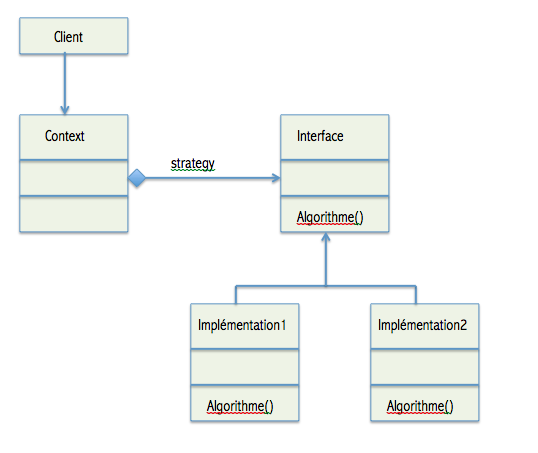
\includegraphics[scale=0.7]{StrategyDesignPattern.png}


Ce pattern est très utile lorsqu'il faut permuter dynamiquement des algorithmes.
Ou par exemple lorsque des classes ne diffèrent que par leur comportement. Ainsi, pour éviter de dupliquer le code, on crée une seule classe comportant les éléments de base ainsi qu'une interface implémentées par diverses classes décrivant les différents comportements de la classe centrale.

De prime abord, il a été pensé de créer pour chacun des fantômes, une interface qui était implémentée par 2 classes : une classe de poursuite et une classe de dispersion.
Or cela engendrait toujours du code dupliqué : les algorithmes de dispersion sont tous les mêmes.

Pour la première version du logiciel, un pattern comme celui qui suit a été crée :

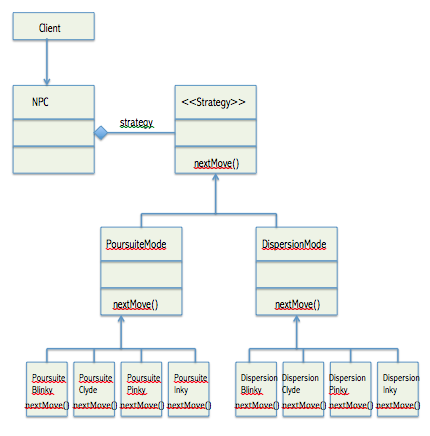
\includegraphics[scale=0.9]{StrategyDP.png}

4 classes associées au mode poursuite pour chaque fantôme ont été crée dans lesquelles la méthode de poursuite a été copié collé. Ces 4 classes héritaient de la classe abstraite PoursuiteMode.
4 autres classes ont vu le jour représentant le mode dispersion de chaque fantôme.
Ces 4 classes héritaient de la classe abstraite DispersionMode.
Et enfin, PoursuiteMode et DispersionMode implémentaient l'interface Strategy.

Pour la 2ème version du logiciel, l'algorithme de dispersion a été crée.
Afin de pouvoir l'exécuter, des variables d'instance ont été aménagé dans la classe Ghost. Un string atteintHome indique si le fantôme a atteint sa case maison (la case du coin), un tableau de directions mémorise le chemin qu'il devra emprunter après avoir visité sa case maison. Un autre tableau de directions représente le chemin qu'il doit prendre à la prochaine occurence et enfin un square représentant sa case "maison".
Cet algorithme est placé dans la classe DispersionMode. Les classes filles font appel à cette même méthode.

La 3ème version, nous avons mis en place la variable strategy nous permettant de jongler entre la dispersion et la poursuite.
Ainsi, un String est placé dans la classe NPC représentant la stratégie en cours : ModeDispersion ou ModePoursuite. Lorsque la stratégie change,au cours du temps, cette variable est modifiée grâce à setStrategy.
Ainsi la méthode nextMove() de blinky par exemple appelle directement la méthode de sa classe de dispersion ou sa classe de poursuite associée en fonction de la valeur de cette variable.
Par conséquent, si l'on souhaite modifier la stratégie d'un fantôme, nous n'avons plus à changer le code dans toutes les classes fantômes mais à rectifier les appels aux méthodes.

Enfin, pour la 4ème et dernière version du logiciel, nous avons indiqué au programme de permuter entre les 2 stratégies en fonction du temps.
Dans la classe NpcMoveTask, une variable temps est crée pour suivre l'écoulement du temps. Celle-ci est incrémentée à chaque occurence de la fonction run de la moyenne d' intervalle entre 2 coups d'un fantôme. 
Dans la fonction run, en fonction de la valeur de cette variable, nous appelons la méthode setStrategy de la classe NPC afin de switcher la stratégie des fantômes.

\section{Fonctionnalités supplémentaires}


\end{document}
